\documentclass[UTF8]{ctexart}
\usepackage{graphicx}
\usepackage{multirow}
\usepackage{booktabs}
\usepackage{indentfirst}
\setlength{\parindent}{2em}
\usepackage{color}
\definecolor{lbcolor}{rgb}{0.9,0.9,0.9}
\usepackage{listings}
\lstset{backgroundcolor=\color{lbcolor}}
\lstset{keywordstyle=\color[rgb]{0,0,1}}
\lstset{commentstyle=\color[rgb]{0.133,0.545,0.133}}
\lstset{stringstyle=\color[rgb]{0.627,0.126,0.941}}
\lstset{language=Matlab}
\lstset{numbers=left}
\lstset{breaklines=true}
\author{何舜成}
\title{系统工程导论第二次作业}
\begin{document}
\maketitle
\section{计算结果}
运行得到的原始数据、回归直线和置信边界如下图:\par
\begin{figure}[htbp]
  \centering
  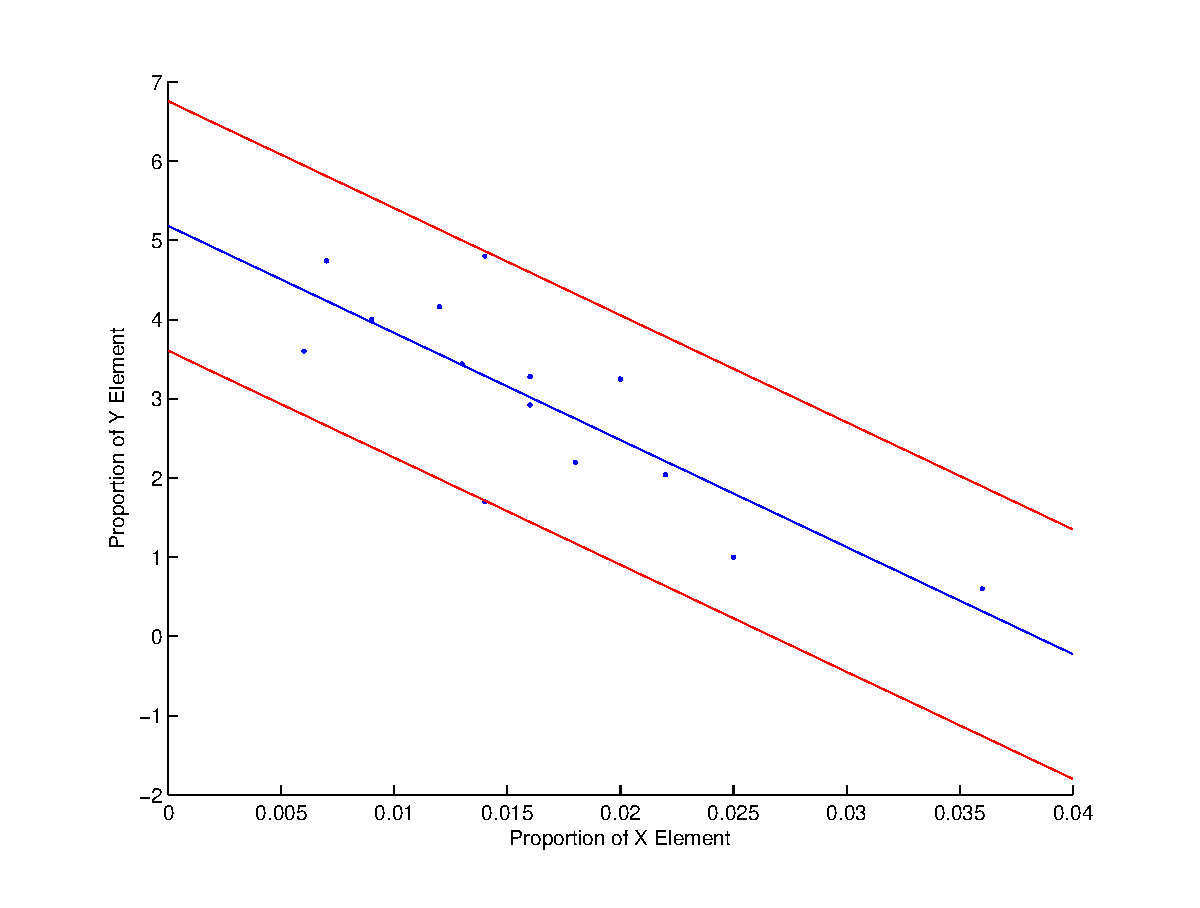
\includegraphics[width=1.05\textwidth]{slot.eps}
\end{figure}
\par
其中回归方程为:\par
\begin{equation}
y = 5.180451 - 135.071531x
\end{equation}
\par
边界方程为:\par
\begin{equation}
y = 6.755133 - 135.071531x
\end{equation}
\par
和\par
\begin{equation}
y = 3.605768 - 135.071531
\end{equation}
\par
14个数据点中有13个点在置信区间内,一个点稍超出置信区间边界。\par
F检验得:\par
\begin{equation}
F=\frac{(N-2)ESS}{RSS}=22.5791
\end{equation}
\begin{equation}
F_{\alpha}=4.7472
\end{equation}
\begin{equation}
F>F_{\alpha}
\end{equation}
\par
拒绝$H_{0}$,即接受$H_{1}$:X和Y呈线性关系(显著性水平$\alpha=0.05$)。\par
\section{具体实现}
Matlab代码(.m文件)如下所示:\par
\begin{lstlisting}
%%
% Input data
%data = [0.009 4.0; 0.013 3.44; 0.006 3.6; 
%    0.025 1.0; 0.022 2.04; 0.007 4.74; 
%    0.036 0.6; 0.014 1.7; 0.016 2.92; 
%    0.014 4.8; 0.016 3.28; 0.012 4.16; 
%    0.020 3.25; 0.018 2.2];
%alpha = 0.05;
%%
function linear_regression1(data, alpha)
%Scatter figure
sz = size(data);
N = sz(1);
x = transpose(data(:,1));% data of x-axis
y = transpose(data(:,2));% data of y-axis
scatter(x,y,'.');
xlabel('Proportion of X Element');
ylabel('Proportion of Y Element');
hold on;
% Calculate the regression equation
avgX = mean(x);
avgY = mean(y);
X = x - avgX;% Move data average to zero
Y = y - avgY;% Move data average to zero
LXY = dot(X,Y);
LXX = dot(X,X);
bhat = LXY / LXX;% Estimated value of slope
ahat = avgY - bhat * avgX;% Estimated value of intersection
% Plot the regression equation
cx = [0:0.001:0.040];
cy = ahat + bhat * cx;
plot(cx,cy);
hold on;
% F-test
Yhat = ahat + bhat * x;% Estimated value regard to regression equation
TSS = dot(Y,Y);% Total square sum
ESS = dot(Yhat-avgY,Yhat-avgY);% Explanation square sum
RSS = TSS - ESS;% Residues
F = (N-2)*ESS/RSS;
Fa = finv(1-alpha,1,N-2);
if F<=Fa
    fprintf('No linear relation! (p=0.95)\n');
else
    fprintf('Linear relation! (p=0.95)\n');
end
% Bounds of confidence interval
sdelta = sqrt(RSS/(N-2));
Z = norminv(1-alpha/2,0,1) * sdelta;
cy1 = ahat + Z + bhat * cx;
cy2 = ahat - Z + bhat * cx;
plot(cx, cy1, 'r');
hold on;
plot(cx, cy2, 'r');
end
\end{lstlisting}
\end{document}